\documentclass[a4paper, 10pt]{article}
\linespread{1.33}
% ┌─────────────────────┐
% │     preamble.tex    │
% └─────────────────────┘

% ══════════ [1] Basic document settings ══════════
\usepackage{fullpage}
\usepackage{geometry}
\geometry{
    top = 2cm,
    bottom = 4.5cm,
    left = 2.5cm,
    right = 2.5cm
}
\usepackage{lastpage}

\usepackage{xcolor}
\usepackage{graphicx}
\usepackage{tikz}
\usepackage{pgfplots}

\usepackage{enumerate}
\usepackage{sectsty}
\subsectionfont{\color{blue}}
\usepackage{enumitem}
\usepackage{array}
\newcolumntype{P}[1]{>{\centering\arraybackslash}p{#1}}

\usepackage{fourier-orns}
\usetikzlibrary{decorations.text}
\pgfplotsset{compat = newest}
\newcommand{\seprule}{
    \vspace*{1.5em}
    \vspace{-8pt}\hrulefill
    \raisebox{-2.1pt}{\quad\decofourleft\decotwo\decofourright\quad}\hrulefill
    \vspace*{1.5em}
}

\usepackage{hyperref}
\hypersetup{
  colorlinks=true,
  linkcolor=blue,
  linkbordercolor={0 0 1},
  urlcolor=blue
}

\usepackage{fancyhdr}
\usepackage[]{mdframed}

\renewcommand{\thesubsection}{\S{} \arabic{section}.\arabic{subsection}}

% ══════════ [2] Math packages ══════════
\usepackage{amsmath}
\usepackage{amsthm}
\usepackage{amsfonts}
\usepackage{amssymb}
\usepackage{amscd}
\usepackage{mathrsfs}
\usepackage{cancel}

% ══════════ [3] Miscellaneous & Fonts ══════════
\setlength{\parindent}{0.0in}
\setlength{\parskip}{0.05in}
\renewcommand{\footrulewidth}{0.4pt}

\usepackage{mathpazo}
\usepackage{domitian}
\usepackage[T1]{fontenc}
\let\oldstylenums\oldstyle
\setmonofont[Scale = 0.8]{DejaVu Sans Mono}

% ══════════ [4] amsthm setup ══════════

\newtheorem{theorem}{Theorem}[section]
\newtheorem{corollary}[theorem]{Corollary}
\newtheorem{lemma}[theorem]{Lemma}

\theoremstyle{definition}
\newtheorem{definition}[theorem]{Definition}

\theoremstyle{remark}
\newtheorem*{remark}{Remark}

\theoremstyle{definition}
\newtheorem{obs}[theorem]{Observation}

\theoremstyle{definition}
\newtheorem{exercise}[theorem]{Exercise}
\newmdtheoremenv[innertopmargin = 8pt,
                 innerbottommargin = 10pt]{exer}[theorem]{Exercise}

\theoremstyle{definition}
\newtheorem{example}[theorem]{Example}
% ┌─────────────────────┐
% │   usercommand.tex   │
% └─────────────────────┘

% ══════════ [1] short-hand notations ══════════
\newcommand{\mbf}{\mathbf}
\newcommand{\mrm}{\mathrm}
\newcommand{\mca}{\mathcal}
\newcommand{\msc}{\mathsc}
\newcommand{\mbb}{\mathbb}
\newcommand{\msf}{\mathsf}

\newcommand{\tbf}{\textbf}
\newcommand{\tit}{\textit}

\newcommand{\eps}{\epsilon}
\newcommand{\kB}{k_{\mathrm{B}}}
\def\dbar{{\mathchar'26\mkern-12mu d}}
\newcommand{\contradiction}{\ensuremath{{\Rightarrow\mspace{-2mu}\Leftarrow}}}
\newcommand{\im}{\mathrm{im}\,}
\renewcommand{\d}{\mathrm{d}}

\renewcommand\qedsymbol{$\blacksquare$}

\newcommand\lecturenumber{08}
\newcommand\lecturedate{Nov 29, 2024}

\pagestyle{fancyplain}
\headheight 40pt
\lhead{Lecture \lecturenumber\\CNBC Deep Learning Subgroup}
\rhead{Riemannian Geometry for Deep Learning \\\lecturedate}
\cfoot{Fall 2024, SNU}
\rfoot{\small\thepage}
\headsep 1.5em

\begin{document}
\setcounter{section}{5}
\section{Lie Derivatives}

\setcounter{subsection}{1}
\subsection{Lie Derivatives (cont'd)}

\setcounter{theorem}{8}

\begin{exer}
    Show that the Lie bracket satisfies ($c_{1},c_{2} \in \mbb{R},\, X_{1},X_{2},Y_{1},Y_{2},X,Y,Z \in \mathscr{X}(\mca{M})$)
    \begin{itemize}
        \item[(a)] bilinearity:
        \begin{align*}
            [X, c_{1}Y_{1} + c_{2}Y_{2}] &= c_{1}[X, Y_{1}] + c_{2}[X, Y_{2}] \\
            [c_{1}X_{1} + c_{2}X_{2}, Y] &= c_{1}[X_{1}, Y] + c_{2}[X_{2}, Y]
        \end{align*}
        \item[(b)] skew-symmetry: $[X, Y] = -[Y, X]$
        \item[(c)] the \tbf{Jacobi identity} $[[X, Y],Z] + [[Z, X], Y] + [[Y, Z], X] = 0$.
    \end{itemize}
\end{exer}

\begin{proof}
    Straightforward.
\end{proof}

\begin{exer}
    Let $X, Y \in \mathscr{X}(\mca{M})$ be vector fields on $\mca{M}$. Show that
    \begin{itemize}
        \item[(a)] For $f \in \mca{F}(\mca{M})$,
        \[ \mca{L}_{fX}Y = f[X, Y] - Y[f]X \;\text{and}\; \mca{L}_{X}(fY) = f[X, Y] + X[f]Y\]
        \item[(b)] For $f \,:\, \mca{M} \rightarrow \mca{N}$,
        \[ f_{\ast}[X, Y] = [f_{\ast}X, f_{\ast}Y] \]
    \end{itemize}
\end{exer}

\begin{proof}
    \begin{itemize}
        \item[(a)] For $g \in \mca{F}(\mca{M})$,
        \begin{align*}
            \mca{L}_{fX}Y[g] &= fX[Y[g]] - Y[fX[g]] = fX[Y[g]] - Y[f]X[g] - fY[X[g]] = (f[X,Y] - Y[f]X)[g] \\
            \mca{L}_{X}(fY)[g] &= X[fY[g]] - fY[X[g]] = X[f]Y[g] + fX[Y[g]] - fY[X[g]] = (f[X,Y] + X[f]Y)[g]
        \end{align*}
        \item[(b)] Let $x^{\mu}$ and $y^{\nu}$ denote the local coordinates in $\mca{M}$ and $\mca{N}$, respectively. In this setup,
        \begin{align*}
            f_{\ast}[X,Y] &= f_{\ast}\left(X^{\mu}\frac{\partial}{\partial x^{\mu}}Y^{\nu} - Y^{\mu}\frac{\partial}{\partial x^{\mu}}X^{\nu}\right)\frac{\partial}{\partial x^{\nu}} \\
            &= \left(X^{\mu}\frac{\partial}{\partial x^{\mu}}Y^{\nu} - Y^{\mu}\frac{\partial}{\partial x^{\mu}}X^{\nu}\right)\frac{\partial y^{\lambda}}{\partial x^{\nu}} \cdot e_{\lambda} \quad (\leftarrow \; e_{\lambda} = \frac{\partial}{\partial x^{\lambda}})
        \end{align*}
        Since
        \[ f_{\ast}X = \underbrace{\left[X^{\nu}\frac{\partial y^{\alpha}}{\partial x^{\nu}}\right]}_{(f_{\ast}X)^{\alpha}}\frac{\partial}{\partial y^{\alpha}} \;\text{and}\; f_{\ast}Y = \underbrace{\left[Y^{\mu}\frac{\partial y^{\beta}}{\partial x^{\mu}}\right]}_{(f_{\ast}X)^{\beta}}\frac{\partial}{\partial y^{\beta}} \]
        we have
        \begin{align*}
            f_{\ast}[X, Y] &= \left[ X^{\mu} \frac{\textcolor{red}{\partial y^{\alpha}}}{\partial x^{\mu}} \cdot \frac{\partial}{\textcolor{red}{\partial y^{\alpha}}} \left((f_{\ast}Y)^{\beta}\frac{\partial x^{\nu}}{\partial y^{\beta}}\right) - Y^{\mu} \frac{\textcolor{red}{\partial y^{\alpha}}}{\partial x^{\mu}} \cdot \frac{\partial}{\textcolor{red}{\partial y^{\alpha}}} \left((f_{\ast}X)^{\beta}\frac{\partial x^{\nu}}{\partial y^{\beta}}\right) \right]\frac{\partial y^{\lambda}}{\partial x^{\nu}} \cdot e_{\lambda} \\
            &= \left[ (f_{\ast}X)^{\alpha}\frac{\partial}{\partial y^{\alpha}}(f_{\ast}Y)^{\beta} - (f_{\ast}Y)^{\alpha}\frac{\partial}{\partial y^{\alpha}}(f_{\ast}X)^{\beta}  \right] \underbrace{\frac{\partial x^{\nu}}{\partial y^{\beta}}\frac{\partial y^{\lambda}}{\partial x^{\nu}}}_{=\delta_{\beta}{}^{\lambda}} \cdot e_{\lambda} \\
            & \qquad\qquad\qquad +\left[ \cancel{(f_{\ast}X)^{\alpha}(f_{\ast}Y)^{\beta}\frac{\partial^{2}x^{\nu}}{\partial y^{\alpha}\partial y^{\beta}}} - \cancel{(f_{\ast}Y)^{\alpha}(f_{\ast}X)^{\beta}\frac{\partial^{2}x^{\nu}}{\partial y^{\alpha}\partial y^{\beta}}} \right]\frac{\partial y^{\lambda}}{\partial x^{\nu}} \cdot e_{\lambda} \\
            &= [f_{\ast}X, f_{\ast}Y]
        \end{align*}
    \end{itemize}
\end{proof}

\begin{obs}[Geometrical meaning of Lie brackets]
    \begin{align*}
        \text{Lie bracket} \quad &= \quad \text{non-commutativity of two flows} \\
        &= \quad \text{failure of the closure of the parallelogram.}
    \end{align*}

    \begin{figure*}[htbp]
        \centering
        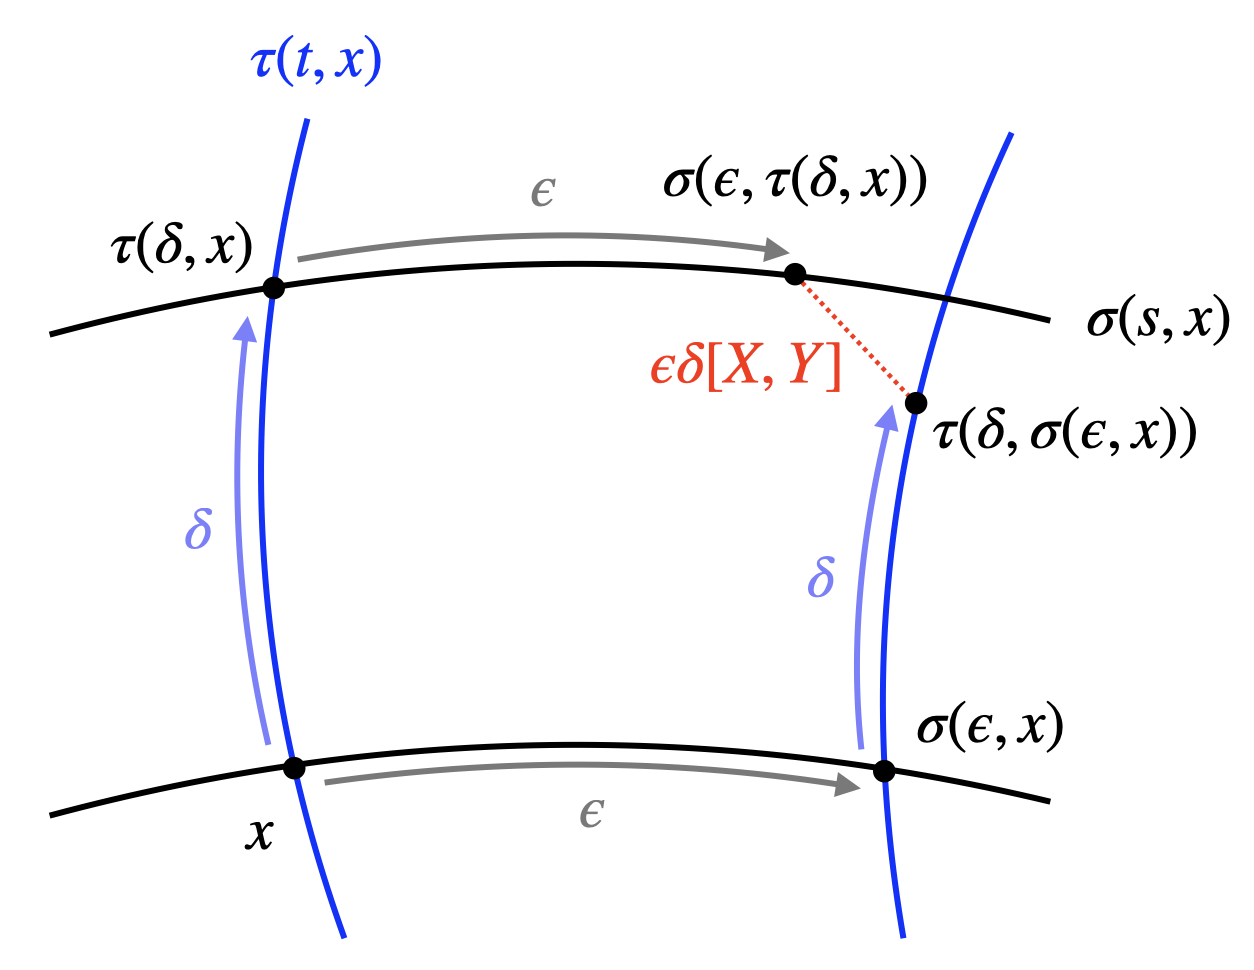
\includegraphics[width = 0.5\textwidth]{../images/lecture08/8_01.png}
    \end{figure*}
    
    Consider two flows $\sigma(s, x)$ and $\tau(t, x)$ generated from $X, Y \in \mathscr{X}(\mca{M})$, respectively. Suppose that we move for $\eps$ along $\sigma$ and then move for $\delta$ along $\tau$.
    \begin{align*}
        \tau^{\mu}(\delta, \sigma(\eps, x)) &\simeq \tau^{\mu}(\delta, x^{\nu} + \eps X^{\nu}(x)) \\
        &\simeq x^{\mu} + \eps X^{\mu}(x) \delta Y^{\mu}(x^{\nu} + \eps X^{\nu}(x)) \\
        &\simeq x^{\mu} + \eps X^{\mu}(x) + \delta Y^{\mu}(x) + \eps\delta X^{\nu}(x)\partial_{\nu}Y^{\mu}(x)
    \end{align*}
    If we go for $\delta$ along $\tau$ first (and $\eps$ along $\sigma$ later),
    \[ \sigma^{\mu}(\eps, \tau(\delta, x)) \simeq x^{\mu} + \eps X^{\mu}(x) + \delta Y^{\mu}(x) + \eps\delta Y^{\nu}(x)\partial_{\nu}X^{\mu}(x) \]
    The \tit{failure} of closure is
    \[ \tau^{\mu}(\delta, \sigma(\eps, x)) - \sigma^{\mu}(\eps, \tau(\delta, x)) = \eps\delta(X^{\nu}\partial_{\nu}Y^{\mu} - Y^{\nu}\partial_{\nu}X^{\mu}) = \boxed{\eps\delta[X,Y]^{\mu}} \]
\end{obs}

\begin{remark}
    \[ \mca{L}_{X}Y = [X, Y] = 0 \quad\Longleftrightarrow\quad \sigma(s, \tau(t, x)) = \tau(t, \sigma(s, x)) \]
    In other words, if two flows commute then Lie derivative vanishes.
\end{remark}
\newpage

% ===== ===== ===== ===== ===== ===== ===== ===== ===== ===== ===== ===== ===== ===== 

\begin{definition}[Lie derivative of one-forms]
    The \tbf{Lie derivative of an one-form} $\omega \in \Omega^{1}(\mca{M})$\footnote{$\Omega^{1}(\mca{M}) \equiv T_{p}^{\ast}(\mca{M})$.} along $X \in \mathscr{X}(\mca{M})$ is defined by
    \[ \mca{L}_{X}\omega = \lim_{\eps\rightarrow 0}\frac{1}{\eps}[(\sigma_{\eps})^{\ast}\omega|_{\sigma_{\eps}(x)} - \omega|_{x}] \]
    where $(\sigma_{\eps})^{\ast}\,:\,T_{\sigma_{\eps}(x)}^{\ast}\mca{M} \rightarrow T_{x}^{\ast}\mca{M}$ is a \tit{pullback} map of $\sigma_{\eps}$.\footnote{As the pushforward maps a vector from one tangent space to the other, pullback maps an one-form from one cotangent space to the other.}
\end{definition}

\begin{obs}
    Put $\omega = \omega_{\mu}\d{x}^{\mu}$. Then
    \[ \omega|_{\sigma_{\eps}(x)} \simeq \omega_{\mu}(x^{\nu} + \eps X^{\nu}(x))\,\d{x}^{\mu}|_{x+\eps X} \simeq [\omega_{\mu}(x) + \eps X^{\nu}(x)\partial_{\nu}\omega_{\mu}(x)]\,\d{x}^{\mu}|_{x + \eps X} \]
    Applying the pullback map gives
    \begin{align*}
        (\sigma_{\eps})^{\ast}\omega|_{\sigma_{\eps}(x)} &= [\omega_{\mu}(x) + \eps X^{\nu}(x)\partial_{\nu}\omega_{\mu}(x)] \underbrace{\frac{\partial(\sigma_{\eps}(x))^{\alpha}}{\partial x^{\mu}}}_{=\partial_{\mu}(x^{\alpha} + \eps X^{\alpha}(x)}\,\d{x}^{\mu}|_{x} \\
        &= \omega_{\mu}\d{x}^{\mu} + \eps[X^{\nu}(x)\partial_{\nu}\omega_{\mu}(x) + \omega_{\nu}(x)\partial_{\mu}X^{\nu}(x)]\,\d{x}^{\mu} + \mca{O}(\eps^{2})
    \end{align*}
    which leads to
    \[ \boxed{\mca{L}_{X}\omega = (X^{\nu}\partial_{\nu}\omega_{\mu} + \partial_{\mu}X^{\nu}\omega_{\nu})\,\d{x}^{\mu}} \in T_{x}^{\ast}\mca{M} \]
\end{obs}

\begin{obs}[Lie derivative of smooth functions]
    The \tbf{Lie derivative of smooth function} $f \in \mca{F}(\mca{M})$ along a flow $\sigma$ generated by a vector field $X$ is
    \begin{align*}
        \mca{L}_{X}f &= \lim_{\eps\rightarrow 0}\frac{1}{\eps}[f(\sigma_{\eps}(x)) - f(x)] = \lim_{\eps\rightarrow 0}\frac{1}{\eps}[f(x^{\mu} + \eps X^{\mu}) - f(x)] \\
        &= X^{\mu}\partial_{\mu}f = X[f]
    \end{align*}
    the usual directional derivative.
\end{obs}

\seprule

How can we compute the Lie derivative of \tit{general} $(q,r)$-tensors?

\begin{prop}
    The Lie derivative satisfies $\mca{L}_{X}(t_{1} + t_{2}) = \mca{L}_{X}t_{1} + \mca{L}_{X}t_{2}$ where $t_{1}$ and $t_{2}$ are tensor fields of the same type. For any type of tensors $t_{1}$ and $t_{2}$, the following holds.
    \[ \mca{L}_{X}(t_{1} \otimes t_{2}) = \mca{L}_{X}t_{1} \otimes t_{2} + t_{1} \otimes \mca{L}_{X}t_{2} \]
\end{prop}

\begin{proof}
    We do not prove this proposition here - instead, we \tit{embrace} it.
\end{proof}
\newpage

% ===== ===== ===== ===== ===== ===== ===== ===== ===== ===== ===== ===== ===== ===== 

\begin{example}
    Take $Y \in \mathscr{X}(\mca{M})$, $\omega \in \Omega^{1}(\mca{M})$ and construct $Y \otimes \omega$. The Lie derivative of this (1,1)-tensor is
    \begin{align*}
        \mca{L}_{X}(Y \otimes \omega) &= \lim_{\eps\rightarrow 0}\frac{1}{\eps}[\{(\sigma_{-\eps}(x))_{\ast}Y \otimes (\sigma_{\eps})^{\ast}\omega\}_{\sigma_{\eps}(x)} - (Y \otimes \omega)|_{x}] \\
        &= \lim_{\eps\rightarrow 0}\frac{1}{\eps}[(\sigma_{-\eps})_{\ast}Y \otimes \{ (\sigma_{\eps})^{\ast}\omega - \omega \} + \{ (\sigma_{-\eps})_{\ast}Y - Y \} \otimes \omega] \\
        &= Y \otimes \mca{L}_{X}\omega + \mca{L}_{X}Y \otimes \omega
    \end{align*}
    For the general (1,1)-tensor $\displaystyle{ T = T_{\mu}{}^{\nu}\,\d{x}^{\mu}\otimes\frac{\partial}{\partial x^{\nu}} \in \mathfrak{T}^{(1,1)}(\mca{M}) }$,
    \[ \mca{L}_{X}T = X[T_{\mu}{}^{\nu}]\,\d{x}^{\nu}\otimes\frac{\partial}{\partial x^{\nu}} + T_{\mu}{}^{\nu}(\mca{L}_{X}\d{x}^{\mu})\otimes\frac{\partial}{\partial x^{\nu}} + T_{\mu}{}^{\nu} \,\d{x}^{\mu}\otimes\left(\mca{L}_{X}\frac{\partial}{\partial x^{\nu}}\right) \]
\end{example}

\begin{exer}
    Let $T$ be a tensor field. Show that
    \[ \mca{L}_{[X, Y]}T = \mca{L}_{X}\mca{L}_{Y}T - \mca{L}_{Y}\mca{L}_{X}T \]
\end{exer}

\begin{proof}
    First, note that
    \[ [X, Y]T = XYT - YXT = XYT - YTX + YTX - YXT = [X, YT] - Y[X, T] \]
    Then
    \begin{align*}
        \mca{L}_{[X,Y]}T &= [[X,Y],T] = [X,Y]T - T[X,Y] \\
        &= [X, YT] - Y[X,T] - [X, TY] - [X,T]Y \\
        &= XYT - YTX - Y[X,T] - XTY + TYX + [X,T]Y \\
        &= X[Y, T] - [Y, T]X + [X, T]Y - Y[X, T] \\
        &= [X, [Y, T]] - [Y, [X, T]] = \boxed{\mca{L}_{X}\mca{L}_{Y}T - \mca{L}_{Y}T\mca{L}_{X}T}
    \end{align*}
\end{proof}

\end{document}
